\documentclass[../main.tex]{subfiles}
\begin{document}
\chapter{2022-2023学年微积分（一）（下）期中考试}

\section{基本计算题(每小题 6 分，共 60 分)}
\begin{enumerate}
    \item 已知$y_{1}=x+\cos x$，$y_{2}=x+\sin x$，$y_{3}=x$是某个二阶常系数非齐次线性微分方程的三个解，求该微分方程及其通解.
          \vspace{10em}

    \item 已知单位向量$\overrightarrow{OA}$与三个坐标轴正向的夹角相等，$\overrightarrow
              {OA}$的方向余弦为正，点$B$是点$M(1,-2,2)$关于点$N(-1,2,1)$的对称点，求以$\overrightarrow
              {OA}$与$\overrightarrow{OB}$为邻边的平行四边形的面积.
          \vspace{11em}

    \item 求二重极限$\lim_{\substack{x\to a \\ y\to 0}}\frac{\sin xy}{y}$，其中$a$为常数.
          \vspace{11em}

    \item 求球面$x^{2}+y^{2}+z^{2}=50$与锥面$x^{2}+y^{2}=z^{2}$所截出的曲线在$(3,
              4,5)$处的切线与法平面方程.
          \vspace{13em}

    \item 设函数$z=z(x,y)$由方程$(z+y)^{x}=x+2y$确定，求$\left.\mathrm{d}z\right|
              _{(1,2)}$.
          \vspace{13em}

    \item 设$u=f(x,y,z)$，$\varphi\left(x^{2},\mathrm{e}^{y},z\right)=0$，$y=\cos
              x$，其中$f$，$\varphi$具有一阶连续偏导数，且$\frac{\partial \varphi}{\partial
                  z}\neq 0$，求$\frac{\mathrm{d}u}{\mathrm{d}x}$.
          \vspace{13em}

    \item 设$f(x,y)=\frac{x^{2}}{2}+\frac{y^{2}}{3}-\frac{4}{\pi}\iint\limits_{D}
              f(x,y)\,\mathrm{d}x\,\mathrm{d}y$，其中平面区域$D=\{(x,y)|x^{2}+y^{2}\leq 1\}$，$f
              (x,y)$为区域$D$上的连续函数，求$f(x,y)$.
          \vspace{12em}

    \item 求积分$I=\int_{-1}^{1}\,\mathrm{d}x\int_{-1}^{x}x\sqrt{1-x^{2}+y^{2}}\,\mathrm{d}
              y$.
          \vspace{11em}

    \item 设函数$z=f\left(x^{2}-y,\varphi(xy)\right)$，其中$f(u,v)$具有二阶连续的偏导数，$\varphi
              (u)$二阶可导，试求$\frac{\partial^{2} z}{\partial x \partial y}$.
          \vspace{11em}

    \item 设平面区域$D=\{(x,y)|x^{2}+y^{2}\leq 1,x^{2}+y^{2}\geq 2y,x^{2}+y^{2}\geq
              -2y, x\geq0\}$，求二重积分$I=\iint\limits_{D}\left(y^{3}+\sqrt{x^{2}+y^{2}}
              \right)\,\mathrm{d}x\,\mathrm{d}y$.
          \vspace{11em}
\end{enumerate}

\section{综合题(每小题 8 分，共 40 分)}
\begin{enumerate}
    \setcounter{enumi}{10}
    \item 设函数$f(u)$具有二阶连续导数，$z=f\left(\mathrm{e}^{x}\cos y\right
              )$满足
          \[
              \frac{\partial^{2} z}{\partial x^{2}}+\frac{\partial^{2} z}{\partial y^{2}}
              =\left(4z+\mathrm{e}^{x}\cos y\right)\mathrm{e}^{2x}.
          \]
          若$f(0)=0$，$f'(0)=0$，求$f(x)$的表达式.
          \vspace{10em}

    \item 求直线$L:
              \begin{cases}
                  x+y+z-1=0, \\
                  2x+y+4z-2=0
              \end{cases}$在曲面$xy+z=0$的点$P_{0}(2,1,-2)$处切平面上的投影直线的方程.
          \vspace{11em}

    \item 设曲面$\Sigma$为曲线$\begin{cases}
                  3x^{2}+2y^{2}=12, \\
                  z=0
              \end{cases}$绕$y$轴旋转一周得到的旋转曲面，求函数$u=z^{4}-3xz+x^{2}+y^{2}$沿$\Sigma$上点$P
              \left(0,\sqrt{3},\sqrt{2}\right)$处指向外侧的法向量方向的方向导数.
          \vspace{11em}

    \item 讨论函数$f(x,y)=
              \begin{cases}
                  \frac{\sqrt{|xy|}\sin(x^{2}+y^{2})}{x^{2}+y^{2}}, & (x,y)\neq (0,0), \\
                  0,                                                & (x,y)=(0,0)
              \end{cases}$在原点$(0,0)$处的连续性、偏导数存在性及可微性.
          \vspace{11em}

    \item 设$P_{0}(x_{0},y_{0},z_{0})$为光滑曲面$S:\varphi(x,y,z)=0$外的一固定点，$P
              (x,y,z)$为$S$上任意一点. 证明：若$\left|\overrightarrow{P_0P}\right|$最短，则$\overrightarrow
              {P_0P}$必是曲面$S$在点$P$处的法向量.
          \vspace{11em}
\end{enumerate}

\chapter{2022-2023学年微积分（一）（下）期中考试参考答案}
\section{基本计算题(每小题 6 分，共 60 分)}
\begin{enumerate}
    \item \textbf{Solution}. 由题意可知$y_{1}-y_{3}=\cos x$，$y_{2}-y_{3}=\sin x$是方程对应的齐次方程的两个线性无关的解，

          它们构成了齐次方程的一个基础解系，且齐次方程的特征根为$\pm i$，所以齐次方程为$y
              ''+y=0$.

          设该微分方程的非齐次项为$f(x)$，将特解$y_{3} = x$代入方程$y''+y=f(x)$，得$f
              (x)=x$.

          所以该二阶常系数非齐次线性微分方程为$y''+y=x$，

          其通解为$y = C_{1}\cos x + C_{2}\sin x + x$，其中$C_{1},C_{2}$为任意常数.

    \item \textbf{Solution}. 由题意可知$\overrightarrow{OA}=\frac{1}{\sqrt{3}}(1,
              1,1)$，$\overrightarrow{OB}=(-3,6,0)$.

          所以平行四边形的面积$S=\left|\overrightarrow{OA}\times \overrightarrow{OB}\right
              |=\sqrt{3}\cdot\sqrt{14}=\sqrt{42}$.

    \item \textbf{Solution}.
          \[
              \begin{aligned}
                  \lim_{\substack{x\to a \\ y\to 0}}\frac{\sin xy}{y}= {} & \lim_{\substack{x\to a \\ y\to 0}}\frac{\sin xy}{xy}\cdot x \\
                  = {}                                                    & \lim_{\substack{u\to 0}}\frac{\sin u}{u}\cdot a = a.
              \end{aligned}
          \]

    \item \textbf{Solution}. 设$F(x,y,z) = x^{2}+y^{2}+z^{2}-50$，$G(x,y,z)=x^{2}
              +y^{2}-z^{2}$.

          \textbf{法一} . 因$\frac{\partial (F,G)}{\partial (y,z)}\bigg|_{(3,4,5)}=
              \begin{vmatrix}
                  2y & 2z  \\
                  2y & -2z
              \end{vmatrix}_{(3,4,5)}=\left.-8yz\right|_{(3,4,5)}=-160\neq 0$，

          所以方程组$\begin{cases}
                  F(x,y,z)=0, \\
                  G(x,y,z)=0
              \end{cases}$可以唯一确定两个具有连续导数的隐函数$y=y(x),z=z(x)$.

          方程组$\begin{cases}
                  F(x,y,z) = x^{2}+y^{2}+z^{2}-50=0, \\
                  G(x,y,z)=x^{2}+y^{2}-z^{2}=0
              \end{cases}$两边对$x$求导，得
          \[
              \begin{cases}
                  2x+2y\frac{\mathrm{d}y}{\mathrm{d}x}+2z\frac{\mathrm{d}z}{\mathrm{d}x}= 0, \\[6pt]
                  2x+2y\frac{\mathrm{d}y}{\mathrm{d}x}-2z\frac{\mathrm{d}z}{\mathrm{d}x}= 0.
              \end{cases}
          \]
          解得$\begin{cases}
                  \frac{\mathrm{d}y}{\mathrm{d}x} = -\frac{x}{y}, \\[6pt]
                  \frac{\mathrm{d}z}{\mathrm{d}x} = 0
              \end{cases}$，所以切线的方向向量可取为$4\left(1,\frac{\mathrm{d}y}{\mathrm{d}x}
              ,\frac{\mathrm{d}z}{\mathrm{d}x}\right)_{(3,4,5)}=\left(4,-3,0\right)$，

          切线的方程为$\frac{x-3}{4}=\frac{y-4}{-3}=\frac{z-5}{0}$，

          法平面的方程为$4\cdot(x-3)-3\cdot(y-4)+0\cdot(z-5)=0$，即$4x-3y=0$.

          \textbf{法二}. $\nabla F = (2x,2y,2z)$，$\nabla G = (2x,2y,-2z)$，

          取两个曲面的法向量分别为$\boldsymbol{n}_{F}= \frac{1}{2}\nabla F|_{(3,4,5)}
              = (3,4,5)$，$\boldsymbol{n}_{G}= \frac{1}{2}\nabla G|_{(3,4,5)}= (3,4,-5)$，

          所以切线的方向向量可取为$-\frac{1}{10}\boldsymbol{n}_{F}\times \boldsymbol{n}
              _{G}=
              \begin{vmatrix}
                  \boldsymbol{i} & \boldsymbol{j} & \boldsymbol{k} \\
                  3              & 4              & 5              \\
                  3              & 4              & -5
              \end{vmatrix}
              = (4,-3,0)$，

          切线的方程为$\frac{x-3}{4}=\frac{y-4}{-3}=\frac{z-5}{0}$，

          法平面的方程为$4\cdot(x-3)-3\cdot(y-4)+0\cdot(z-5)=0$，即$4x-3y=0$.

    \item \textbf{Solution}. 将$x=1$，$y=2$代入方程$(z+y)^{x} = x+2y$得$z=3$. 原方程两边全微分，得
          \[
              \begin{aligned}
                  \mathrm{d}\mathrm{e}^{x\ln(z+y)}= {}                                                                   & \mathrm{d}(x+2y)           \\
                  \left(z+y\right)^{x}\,\mathrm{d}\left(x\ln(z+y)\right) = {}                                            & \mathrm{d}x+2\,\mathrm{d}y \\
                  \left(z+y\right)^{x}\left(\ln(z+y)\,\mathrm{d}x+x\cdot \frac{\mathrm{d}z+\mathrm{d}y}{z+y}\right) = {} & \mathrm{d}x+2\,\mathrm{d}y
              \end{aligned}
          \]
          将$x=1,y=2,z=3$代入上式，得$5\left(\ln 5\,\mathrm{d}x+\frac{\mathrm{d}z+\mathrm{d}y}{5}
              \right)=\mathrm{d}x+2\,\mathrm{d}y$，

          整理得$\left.\mathrm{d}z\right|_{(1,2)}= \left(1-5\ln 5\right)\,\mathrm{d}x +
              \mathrm{d}y$.

    \item \textbf{Solution}. 方程$\varphi\left(x^{2},\mathrm{e}^{y},z\right)=0$两边对$x$求导，得
          \[
              \varphi'_{1}\cdot 2x + \varphi'_{2}\cdot \mathrm{e}^{y}\cdot \frac{\mathrm{d}y}{\mathrm{d}x}
              + \varphi'_{3}\cdot \frac{\partial z}{\partial x}= 0,
          \]
          且$\frac{\mathrm{d}y}{\mathrm{d}x}=-\sin x$，所以$\frac{\partial z}{\partial
                  x}= \frac{-2x\varphi'_{1}+\varphi'_{2}\cdot \mathrm{e}^{y}\sin x}{\varphi'_{3}}$.

          从而
          \[
              \frac{\mathrm{d}u}{\mathrm{d}x}=f'_{1}+f'_{2}\cdot \frac{\mathrm{d}y}{\mathrm{d}x}
              +f'_{3}\cdot \frac{\partial z}{\partial x}= f'_{1} - f'_{2}\sin x + f'_{3}\cdot
              \frac{-2x\varphi'_{1}+\varphi'_{2}\cdot \mathrm{e}^{y}\sin x}{\varphi'_{3}}.
          \]

    \item \textbf{Solution}. 设$\iint\limits_{D}f(x,y)\,\mathrm{d}x\,\mathrm{d}y=C$，方程$f
              (x,y)=\frac{x^{2}}{2}+\frac{y^{2}}{3}-\frac{4}{\pi}C$两边在区域$D$上积分，得
          \[
              \begin{aligned}
                  C = {} & \iint\limits_{D}\left(\frac{x^2}{2}+\frac{y^2}{3}\right)\,\mathrm{d}x\,\mathrm{d}y-\frac{4}{\pi}C\iint\limits_{D}\,\mathrm{d}x\,\mathrm{d}y \\
                  = {}   & \frac{5}{12}\iint\limits_{D}\left(x^{2}+y^{2}\right)\,\mathrm{d}x\,\mathrm{d}y-4C                                                           \\
                  = {}   & \frac{5}{12}\int_{0}^{2\pi}\,\mathrm{d}\theta\int_{0}^{1}r^{3}\,\mathrm{d}r-4C                                                              \\
                  = {}   & \frac{5}{12}\cdot \frac{2\pi}{4}-4C = \frac{5}{24}\pi - 4C.
              \end{aligned}
          \]

          解得$C=\frac{1}{24}\pi$，所以$f(x,y)=\frac{x^{2}}{2}+\frac{y^{2}}{3}-\frac{4}{\pi}
              \cdot \frac{1}{24}\pi = \frac{x^{2}}{2}+\frac{y^{2}}{3}-\frac{1}{6}$.

    \item \textbf{Solution}. 积分区域如图所示，其中$D_{1}=\{(x,y)|-1\leq y\leq 0,
              y\leq x\leq -y\}$，

          $D_{2}=\{(x,y)|0 \leq x\leq 1, -x\leq y\leq x\}$. 则$I = \iint\limits_{D_1+D_2}
              x\sqrt{1-x^{2}+y^{2}}\,\mathrm{d}x\,\mathrm{d}y$.\\
          \noindent
          \begin{minipage}[c]{0.65\textwidth}
              由于$D_{1}$关于$y$轴对称，被积函数$y=x\sqrt{1-x^{2}+y^{2}}$关于$x$是奇函数，\\[1em]
              所以$\iint\limits_{D_1}x\sqrt{1-x^{2}+y^{2}}\,\mathrm{d}x\,\mathrm{d}y=0$.

              又$D_{2}$关于$x$轴对称，被积函数$y=x\sqrt{1-x^{2}+y^{2}}$关于$y$是偶函数，

              所以
              \[
                  \begin{aligned}
                      I = {} & \iint\limits_{D_2}x\sqrt{1-x^2+y^2}\,\mathrm{d}x\,\mathrm{d}y = 2\int_{0}^{1}\,\mathrm{d}y\int_{y}^{1}x\sqrt{1-x^2+y^2}\,\mathrm{d}x \\
                      = {}   & -\int_{0}^{1}\left[\left.\frac{2}{3}\left(1-x^{2}+y^{2}\right)^{\frac{3}{2}}\right|_{x=y}^{x=1}\right]\mathrm{d}y                    \\
                      = {}   & -\frac{2}{3}\int_{0}^{1}\left(y^{3}-1\right)\,\mathrm{d}y = -\frac{2}{3}\cdot\left(\frac{1}{4}-1\right) = \frac{1}{2}.
                  \end{aligned}
              \]
          \end{minipage}
          \hfill %
          \begin{minipage}[c]{0.4\textwidth}
              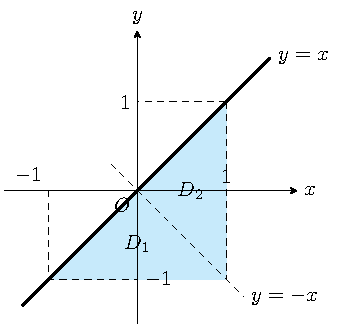
\includegraphics[width=5cm]{2023x-figure1.pdf} % 引入图片源
          \end{minipage}

    \item \textbf{Solution}. $\frac{\partial z}{\partial x}=f'_{1}\cdot 2x+f'_{2}
              \cdot \varphi'(xy)\cdot y$，
          \[
              \begin{aligned}
                  \frac{\partial^2 z}{\partial x \partial y}= {} & \frac{\partial}{\partial y}\left(2xf'_{1} + yf'_{2}\varphi'(xy)\right)                                                                                \\
                  = {}                                           & 2x\left(-f''_{11}+xf''_{12}\varphi'(xy)\right)+f'_{2}\varphi'(xy) + y\varphi'(xy)\left(-f''_{21}+xf''_{22}\varphi'(xy)\right) + xyf'_{2}\varphi''(xy) \\
                  = {}                                           & -2xf''_{11}+\left(2x^{2}-y\right)f''_{12}\varphi'(xy)+f'_{2}\varphi'(xy)+xy\left(f''_{22}\varphi'^{2}(xy)+f'_{2}\varphi''(xy)\right).
              \end{aligned}
          \]
          其中由$f(u,v)$二阶偏导数的连续性可得$f''_{12}=f''_{21}$.

    \item \textbf{Solution}. 积分区域如图所示，由对称性可得$I=\iint\limits_{D}y^{3}
              \mathrm{d}x\,\mathrm{d}y+\iint\limits_{D}\sqrt{x^{2}+y^{2}}\,\mathrm{d}x\,\mathrm{d}
              y = 2\iint\limits_{D_1}\sqrt{x^{2}+y^{2}}\,\mathrm{d}x\,\mathrm{d}y$，

          其中$D_{1}=\{(x,y)|x^{2}+y^{2}\leq 1,x^{2}+y^{2}\geq 2y, x\geq0,y\geq0\}$.\\
          \noindent
          \begin{minipage}[c]{0.65\textwidth}
              用极坐标代换，则
              \[
                  \begin{aligned}
                      I = {} & 2\iint\limits_{D_1}\sqrt{x^2+y^2}\,\mathrm{d}x\,\mathrm{d}y = 2\int_{0}^{\frac{\pi}{6}}\,\mathrm{d}\theta\int_{2\sin \theta}^{1}r^{2}\,\mathrm{d}r                                           \\
                      = {}   & 2\int_{0}^{\frac{\pi}{6}}\left.\frac{r^3}{3}\right|_{2\sin \theta}^{1}\,\mathrm{d}\theta = \frac{2}{3}\int_{0}^{\frac{\pi}{6}}\left(1-8\sin^{3} \theta\right)\,\mathrm{d}\theta              \\
                      = {}   & \frac{\pi}{9}-\frac{16}{3}\int_{0}^{\frac{\pi}{6}}\sin^{3} \theta\,\mathrm{d}\theta = \frac{\pi}{9}+\frac{16}{3}\int_{0}^{\frac{\pi}{6}}\left(1-\cos^{2} \theta\right)\,\mathrm{d}\cos\theta \\
                      = {}   & \frac{\pi}{9}+\frac{16}{3}\left[\cos \theta-\frac{\cos^3 \theta}{3}\right]_{0}^{\frac{\pi}{6}}= \frac{\pi}{9}+\frac{16}{3}\left(\frac{\sqrt{3}}{2}-\frac{\sqrt{3}}{8}-1+\frac{1}{3}\right)   \\
                      = {}   & \frac{\pi}{9}+\frac{16}{3}\cdot\left(\frac{3\sqrt{3}}{8}-\frac{2}{3}\right) = \frac{\pi}{9}-\frac{32}{9}+2\sqrt{3}.
                  \end{aligned}
              \]
          \end{minipage}
          \hfill %
          \begin{minipage}[c]{0.4\textwidth}
              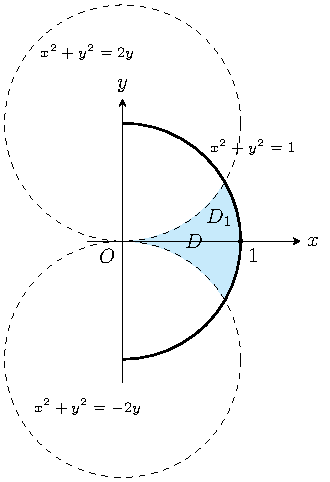
\includegraphics[width=5cm]{2023x-figure2.pdf} % 引入图片源
          \end{minipage}
\end{enumerate}

\section{综合题(每小题 8 分，共 40 分)}
\begin{enumerate}
    \setcounter{enumi}{10}
    \item \textbf{Solution}. $\frac{\partial z}{\partial x}= f'\left(\mathrm{e}
              ^{x}\cos y\right)\cdot \mathrm{e}^{x}\cos y$，$\frac{\partial z}{\partial
                  y}= f'\left(\mathrm{e}^{x}\cos y\right)\cdot \left(-\mathrm{e}^{x}\sin y\right
              )$，

          $\frac{\partial^{2} z}{\partial x^{2}}= f''\left(\mathrm{e}^{x}\cos y\right
              )\cdot \mathrm{e}^{2x}\cos^{2} y + f'\left(\mathrm{e}^{x}\cos y\right)\cdot
              \mathrm{e}^{x}\cos y$，

          $\frac{\partial^{2} z}{\partial y^{2}}= f''\left(\mathrm{e}^{x}\cos y\right
              )\cdot \mathrm{e}^{2x}\sin^{2} y - f'\left(\mathrm{e}^{x}\cos y\right)\cdot
              \mathrm{e}^{x}\cos y$.

          所以
          \[
              \frac{\partial^{2} z}{\partial x^{2}}+\frac{\partial^{2} z}{\partial
                  y^{2}}= f''\left(\mathrm{e}^{x}\cos y\right)\cdot \mathrm{e}^{2x}= \left(4f
              \left(\mathrm{e}^{x}\cos y\right)+\mathrm{e}^{x}\cos y\right)\mathrm{e}^{2x},
          \]
          即$f''(u) = 4f(u)+u$. 齐次方程$f''-4f=0$的特征方程为$r^{2}-4=0$，解得$r=\pm 2$，

          所以齐次方程的通解为$C_{1}\mathrm{e}^{2x}+C_{2}\mathrm{e}^{-2x}$.

          对于$y=x$，$\lambda = 0$不是特征方程的根，故可设特解为$y^{*}=cx$，代入得$0 =
              4cx + x$，解得$c=-\frac{1}{4}$，

          所以非齐次方程的通解为$f(x) = C_{1}\mathrm{e}^{2x}+C_{2}\mathrm{e}^{-2x}-\frac{1}{4}
              x$.

          将$f(0)=0$，$f'(0)=0$代入上式，得$\begin{cases}
                  C_{1}+C_{2}=0, \\
                  2C_{1}-2C_{2}-\frac{1}{4}=0
              \end{cases}$，解得$C_{1}=\frac{1}{16}$，$C_{2}=-\frac{1}{16}$.

          因此$f(x) = \frac{1}{16}\mathrm{e}^{2x}-\frac{1}{16}\mathrm{e}^{-2x}-\frac{1}{4}
              x$.

    \item \textbf{Solution}. 令$F(x,y,z) = xy+z$，$\nabla F = (y,x,1)$，

          则曲面$xy+z=0$在点$P_{0}(2,1,-2)$处切平面的法向量可以取为$\nabla F|_{P_0}= (
              1,2,1)$，

          切平面为$1\cdot(x-2)+2\cdot(y-1)+1\cdot(z+2)=0$，即$x+2y+z=2$.

          设经过直线$L$的平面束方程为$x+y+z-1+\lambda(2x+y+4z-2)=0$，

          即$(2\lambda+1)x + (\lambda+1)y + (4\lambda+1)z - (2\lambda+1)=0$，

          令其与切平面垂直，即$(2\lambda+1, \lambda+1, 4\lambda+1) \cdot (1,2,1) = 8\lambda
              + 4 = 0$，解得$\lambda = -\frac{1}{2}$，

          所以切平面上的投影直线的方程为$\begin{cases}
                  x+2y+z=2, \\
                  y-2z=0.
              \end{cases}$

    \item \textbf{Solution}. 由题意可知曲面$\Sigma$的方程为$3(x^{2}+z^{2})+2
              y^{2}=12$，

          $\nabla \left(3(x^{2}+z^{2})+2y^{2}\right)|_{P}= (6x, 4y, 6z)|_{P}= (0,4\sqrt{3}
              ,6\sqrt{2})$.

          所以$\Sigma$在点$P\left(0,\sqrt{3},\sqrt{2}\right)$处指向外侧的单位法向量$\boldsymbol
              {n}=\left(0,\frac{\sqrt{10}}{5},\frac{\sqrt{15}}{5}\right)$.

          又$\nabla u = (-3z+2x, 2y, 4z^{3}-3x)$，所以$\nabla u|_{P}= \left(-3\sqrt{2}
              , 2\sqrt{3}, 8\sqrt{2}\right)$，

          $\frac{\partial u}{\partial \boldsymbol{n}}= \nabla u|_{P}\cdot \boldsymbol
              {n}= \frac{\sqrt{10}}{5}\cdot 2\sqrt{3}+ \frac{\sqrt{15}}{5}\cdot 8\sqrt{2}
              = 2\sqrt{30}$.

    \item \textbf{Solution}. 因为
          \[
              \lim_{\substack{x\to 0 \\ y\to 0}}\frac{\sqrt{|xy|}\sin\left(x^{2}+y^{2}\right)}{x^{2}+y^{2}}
              =\lim_{\substack{x\to 0 \\ y\to 0}}\frac{\sqrt{|xy|}\cdot\left(x^{2}+y^{2}\right)}{x^{2}+y^{2}}
              = \lim_{\substack{x\to 0 \\ y\to 0}}\sqrt{|xy|}=0=f(0,0),
          \]
          因此函数$f(x,y)$在原点处连续.

          又$f(x,0)=f(0,y)\equiv 0$，所以$f_{x}(0,0)=f_{y}(0,0)=0$，因此函数$f(x,y)$在原点处的偏导数存在.

          考察
          \[
              \lim_{\substack{x\to 0 \\ y\to 0}}\frac{f(x,y)-f(0,0)-f_{x}(0,0)x-f_{y}(0,0)y}{\sqrt{x^{2}+y^{2}}}
              = \lim_{\substack{x\to 0 \\ y\to 0}}\frac{\sqrt{|xy|}\sin\left(x^{2}+y^{2}\right)}{\left(x^{2}+y^{2}\right)\sqrt{x^2+y^2}}.
          \]

          当$y=x,x\to0,y\to0$时，
          \[
              \lim_{\substack{x\to 0 \\ y\to 0}}\sqrt{\frac{|xy|}{x^{2}+y^{2}}}
              = \lim_{x\to0}\sqrt{\frac{x^{2}}{2x^{2}}}= \frac{\sqrt{2}}{2},
          \]
          所以$\lim_{\substack{x\to 0 \\ y\to 0}}
              \frac{\sqrt{|xy|}\sin\left(x^{2}+y^{2}\right)}{\left(x^{2}+y^{2}\right)\sqrt{x^2+y^2}}
              \neq 0$，函数$f(x,y)$在原点处不可微.

    \item \textbf{Solution}. 考虑距离平方函数
          \[
              f(x,y,z) = \left|\overrightarrow{P_0P}\right|^{2} = (x-x_{0})^{2}+(y-y_{0}
              )^{2}+(z-z_{0})^{2},
          \]
          若$P$是$S$上使得$\left|\overrightarrow{P_0P}\right|$最小的点，则等价于$f(x,
              y,z)$在约束条件$\varphi(x,y,z)=0$下取得最小值.

          由于曲面光滑，根据Lagrange乘数法，存在实数$\lambda$使得在点$P$处
          \[
              \nabla f = \lambda \nabla \varphi,
          \]
          其中$\nabla f = 2(x-x_{0}, y-y_{0}, z-z_{0})=2\overrightarrow{P_0P}$，于是得到$\overrightarrow
              {P_0P}= \frac{\lambda}{2}\nabla \varphi$.

          注意到$\nabla \varphi$即为曲面$S$在点$P$处的一个法向量，上式表明$\overrightarrow
              {P_0P}$与$\nabla \varphi$平行，

          所以$\overrightarrow{P_0P}$必然也是曲面$S$在点$P$处的法向量.

\end{enumerate}
\end{document}





